%% ============================================================
%%  Chapter 3: System Design and Methodology
%% ============================================================
\chapter{System Design and Methodology}
\label{chap:methodology}

This chapter describes the full coordination pipeline developed in this thesis.
Section~\ref{sec:method_formulation} establishes the formal problem statement
and notation used throughout.
Section~\ref{sec:method_overview} presents the high-level system architecture.
Section~\ref{sec:method_environment} describes the warehouse simulation environment.
Section~\ref{sec:method_gcbba} details the GCBBA algorithm and its adaptation
to the warehouse setting, culminating in the LCBA extension.
Section~\ref{sec:method_collision} describes the family of three path planning
strategies available within the pipeline.
Section~\ref{sec:method_dynamic} explains the dynamic replanning mechanism
that ties allocation and path execution together.
Section~\ref{sec:method_baselines} describes the baseline methods, and
Section~\ref{sec:method_design} justifies the key architectural decisions.


%% ── 3.1 ─────────────────────────────────────────────────────────
\section{Problem Formulation}
\label{sec:method_formulation}

Let $\mathcal{A} = \{a_1, \ldots, a_{\Na}\}$ denote a team of $\Na$ homogeneous
mobile agents operating on a two-dimensional grid workspace
$\mathcal{W} \subset \mathbb{Z}^2$ containing a set of static obstacles
$\mathcal{O} \subset \mathcal{W}$.
At each discrete timestep $t \in \{0, 1, 2, \ldots\}$, each agent occupies a
unique cell $x_i(t) \in \mathcal{W} \setminus \mathcal{O}$ and may choose to move to any
of its four cardinal neighbours or remain stationary (Hold Position).

\textbf{Tasks.}
Tasks arrive online over time.
Let $\mathcal{T}(t)$ denote the set of tasks available at timestep $t$.
Each task $\tau_j \in \mathcal{T}(t)$ is a pickup-and-delivery pair
$\tau_j = (s_j^{\text{in}}, s_j^{\text{ej}})$, where
$s_j^{\text{in}} \in \mathcal{S}^{\text{in}}$ is the induct (pickup) station and
$s_j^{\text{ej}} \in \mathcal{S}^{\text{ej}}$ is the eject (delivery) station.
A task is \emph{completed} when an agent visits $s_j^{\text{in}}$ followed by
a visit to $s_j^{\text{ej}}$ while the task is assigned to it.
Doing this constitutes completing a task.

\textbf{Communication.}
Agents communicate over a proximity-based wireless channel with range
$\comm > 0$.
The communication graph at time $t$ is
\begin{equation}
  G(t) = (\mathcal{A},\; E(t)),
  \quad
  E(t) = \bigl\{(i,k) : \|x_i(t) - x_k(t)\|_2 \leq \comm\bigr\},
  \label{eq:comm_graph}
\end{equation}
where $\|\cdot\|_2$ denotes Euclidean distance.
The graph $G(t)$ may be disconnected and changes at every timestep as agents
move.

\textbf{Objective.}
The system operates in two experimental modes.
In \emph{batch mode}, a fixed set of $\Nt$ tasks is released at $t = 0$ and
the objective is to minimise makespan: the timestep at which the last task is
completed.
In \emph{steady-state mode}, tasks arrive continuously at each induct station at
rate $\lambda$ tasks per timestep, and the objective is to maximise throughput:
the number of tasks completed per timestep after a warm-up period.

\textbf{Constraints.}
In both modes, every agent must follow a collision-free path:
no two agents may occupy the same cell at the same timestep (vertex conflict),
and no two agents may traverse the same edge in opposite directions within the
same timestep (edge conflict).
Agents have finite energy and must periodically visit a designated charging
station; they may not execute tasks while charging.
All decisions must be made using only information locally available to an agent
within its communication neighbourhood $\mathcal{N}_i(t) = \{k : (i,k) \in E(t)\}$.


%% ── 3.2 ─────────────────────────────────────────────────────────
\section{System Architecture Overview}
\label{sec:method_overview}

The coordination pipeline is structured around two principal components, shown
schematically in Figure~\ref{fig:system_architecture}: a \emph{task allocator}
and a \emph{path planner}, integrated through a centralised
\texttt{IntegrationOrchestrator}.

\begin{figure}[htbp]
  \centering
  % 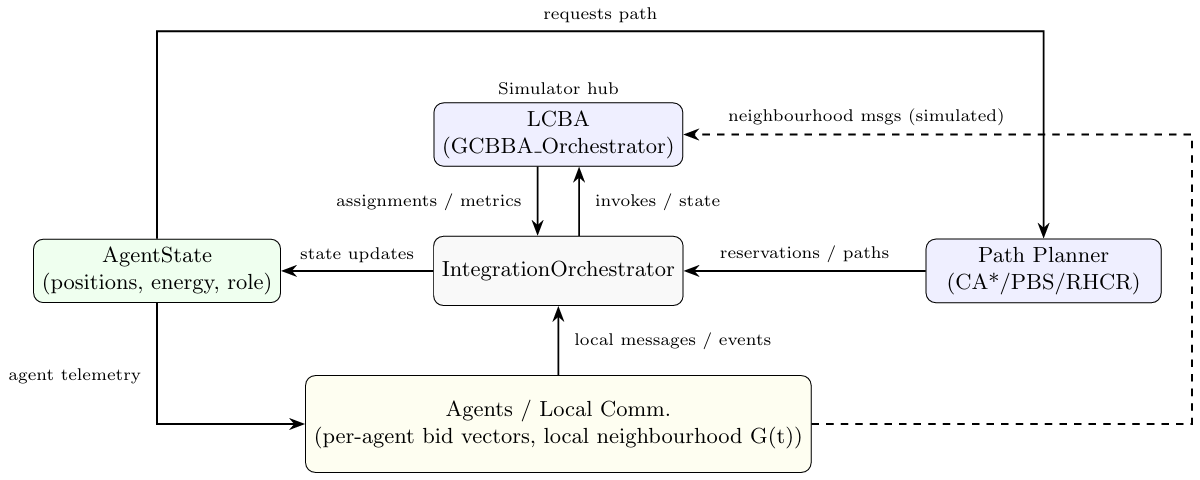
\includegraphics[width=0.9\textwidth]{figures/system_architecture}
  \textbf{[FIGURE PLACEHOLDER: System architecture block diagram showing IntegrationOrchestrator,
  GCBBA\_Orchestrator, PathPlanner, AgentState, and data flow between them.]}
  \caption{System architecture overview. The \texttt{IntegrationOrchestrator}
           coordinates the LCBA task allocator with one of three interchangeable
           path planners. Allocation is logically decentralised (agents run
           the GCBBA protocol using only local communication), while path
           planning uses a shared reservation table maintained by the
           orchestrator.}
  \label{fig:system_architecture}
\end{figure}

The task allocator runs the GCBBA/LCBA algorithm (Section~\ref{sec:method_gcbba}).
It is \emph{logically decentralised}: each agent maintains its own bid and
assignment vectors and communicates only with its current communication
neighbours.
The orchestrator simulates this communication by invoking the GCBBA update
rules for each agent using only the neighbourhood defined by $G(t)$.

The path planner (Section~\ref{sec:method_collision}) is \emph{physically
centralised} in the simulation: the orchestrator has global visibility of
all agent positions and plans collision-free paths for all agents using
a shared space-time reservation table.
% This design choice --- decentralised allocation, centralised collision
% avoidance --- is justified on two grounds.
% First, task allocation decisions are inherently private: agents in disconnected
% components have different information and may reach different allocation
% decisions, which is exactly the behaviour we wish to study.
% Second, collision-free path planning in a bounded warehouse environment does not
% require private information; centralising it eliminates the complexity of
% distributed reservation table consensus while keeping the allocation protocol
% clean for comparison across baselines.
The path planner is designed as a modular component; three implementations are
provided and studied in Section~\ref{sec:method_collision}.

Each agent's state is tracked by an \texttt{AgentState} object that records
its current position, assigned task, planned path, energy level, and charging
status.
The per-timestep simulation loop, described in
Section~\ref{sec:method_dynamic}, drives agents forward along their planned
paths and triggers replanning events as needed.


%% ── 3.3 ─────────────────────────────────────────────────────────
\section{Warehouse Environment}
\label{sec:method_environment}

Experiments are conducted across six warehouse environments of increasing scale,
summarised in Table~\ref{tab:environments}.
Each environment is a 2D gridworld with induct stations (task pickup points),
eject stations (delivery destinations), internal obstacles representing shelving
aisles, and charging stations.
All agents are initialised at their home positions at $t = 0$.

\begin{table}[htbp]
  \centering
  \caption{Warehouse environments used in the evaluation, ordered by fleet size.}
  \label{tab:environments}
  \small
  \begin{tabular}{lccccc}
    \toprule
    \textbf{Environment} & \textbf{Grid} & \textbf{Agents} $\Na$ &
    \textbf{Induct} $|\mathcal{S}^{\text{in}}|$ &
    \textbf{Eject} $|\mathcal{S}^{\text{ej}}|$ \\
    \midrule
    \texttt{warehouse\_small}  & $30\times30$   & 6   & 8  & 38 \\
    \texttt{crossdock}         & $44\times28$   & 12  & 6  & 10 \\
    \texttt{kiva}              & $36\times36$   & 20  & 5  & 10 \\
    \texttt{warehouse\_large}  & $60\times60$   & 18  & 12 & 80 \\
    \texttt{kiva\_large}       & $72\times72$   & 80  & 5  & 10 \\
    \texttt{shelf\_aisle}      & $161\times63$  & 200 & 20 & 19 \\
    \bottomrule
  \end{tabular}
\end{table}

The environments span fleet sizes from 6 to 200 agents and grid areas from
$900$ to over $10{,}000$ cells, enabling evaluation across a wide range of
congestion levels and communication graph densities.
\texttt{warehouse\_small} is used as the primary development and ablation
environment; results across all six environments are reported in the
scalability experiments (Section~\ref{sec:exp_planners}).

\begin{figure}[htbp]
  \centering
  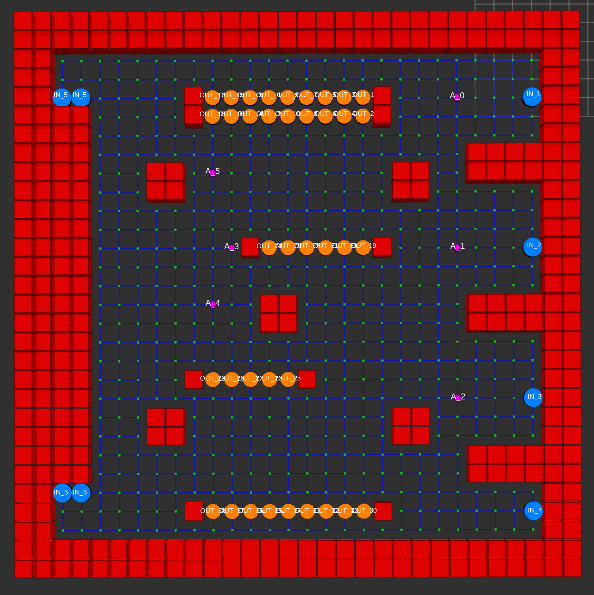
\includegraphics[width=0.6\textwidth]{figures/gridworld_warehouse_small/gridworld_warehouse_small}
  \caption{The \texttt{warehouse\_small} ($30 \times 30$) environment.
           Induct stations (blue) are task pickup locations; eject stations
           (orange) are delivery destinations; obstacles and shelving are
           shown in red; agents are shown in purple.
           Internal shelving creates constrained navigation corridors.}
  \label{fig:gridworld}
\end{figure}

\textbf{Task arrival model.}
In batch mode, all $\Nt$ tasks are injected at $t = 0$.
In steady-state mode, each induct station generates one task every
$\text{round}(1/\lambda)$ timesteps (minimum 1), where $\lambda$ is the
per-station arrival rate.
A per-station queue of depth $Q_{\max} = 5$ buffers tasks before they are
claimed by an agent; tasks that arrive when the queue is full are dropped and
counted as a capacity violation metric.

\textbf{Energy model.}
Each agent starts with full energy $E_{\max}$ and expends one unit per timestep of movement; stationary agents do not consume energy.
The charging trigger condition checks, at every timestep:
\begin{equation}
  \alpha \cdot d_{\text{charger}}(x_i(t)) > e_i(t),
  \label{eq:charge_trigger}
\end{equation}
where $e_i(t)$ is the agent's current energy level,
$d_{\text{charger}}(x_i(t))$ is the BFS shortest-path distance to the
nearest available charging station, and $\alpha \geq 1$ is the
\emph{charging trigger multiplier}.
Setting $\alpha > 1$ introduces a conservative safety margin: the agent
departs for a charger while it still holds more energy than strictly
required for the trip, preventing the degenerate case where an agent runs
out of power en route to the charger and stalls in the middle of the floor.

When the trigger fires, the agent immediately suspends its current task
(which reverts to \textsc{Planned} state and becomes eligible for reassignment),
navigates to the nearest available charging station at highest path-planning
priority, and charges at a configurable rate $\rho_c$ units per timestep
until $e_i = E_{\max}$.
Charging stations are \emph{exclusive}: at most one agent occupies each
station at a time, so the orchestrator assigns agents to distinct stations
and routes subsequent chargers to the next-nearest free station.
Once fully charged, the agent re-enters the allocation pool and a
reallocation event is triggered automatically
(Section~\ref{sec:method_triggers}).

Crucially, energy levels are also incorporated into the bid computation:
before an agent adds a task to its bundle, it checks whether the estimated
travel distance to complete that task exceeds its remaining energy budget.
If so, the task is filtered out of the candidate set.
This \emph{energy-budget filter} prevents agents from winning bids on tasks
they cannot physically complete before needing to recharge, which would
otherwise cause a mid-execution hand-off and wasted travel.

The energy configuration is validated at initialisation: if any reachable
grid position is so far from all chargers that $\alpha \cdot d > E_{\max}$,
an error is raised at startup, guaranteeing that a correctly configured
system can always reach a charger from any occupied cell.

\textbf{Wait stations.}
Idle agents --- those with no current task assignment and not en route to a
charger --- are a source of avoidable congestion: a robot parked in the
middle of a picking aisle forces every active agent to route around it,
adding detours and inflating travel times under high load.
To mitigate this, the system designates a set of \emph{wait stations}
$\mathcal{S}^{\text{wait}}$, configured in the map YAML as
\texttt{idle\_task\_stations}.
Wait stations are placed at low-traffic positions at the periphery of the
grid (typically behind induct stations or at corridor dead-ends) where
parked agents do not interrupt active delivery flows.

When an agent becomes idle and no task is immediately available, the
orchestrator routes it to its nearest unoccupied wait station using the
idle-role path planner.
Wait stations are \emph{exclusively reserved}: the orchestrator maintains a
dynamic reservation set and prevents two agents from targeting the same
station simultaneously; if all stations are occupied, the agent waits in
place.
When a new task is subsequently allocated to the waiting agent, it
immediately preempts its parking navigation and replans toward the task's
induct station, incurring no additional latency.

This behaviour mirrors industrial deployments such as Amazon Robotics and
Ocado, where idle drive units park at designated staging areas to keep main
picking aisles clear for active robots.

\textbf{Distance computation.}
All travel-time estimates used in the GCBBA bid computation
(Section~\ref{sec:method_gcbba}) are derived from BFS-precomputed shortest-path
tables over the obstacle-free grid, not Euclidean distance.
This is crucial: Euclidean distance systematically underestimates travel time
near obstacle clusters, causing agents to bid too aggressively on distant tasks
and producing suboptimal assignments.
The BFS tables are computed once at initialisation and shared across all agents.


%% ── 3.4 ─────────────────────────────────────────────────────────
\section{GCBBA for Warehouse Task Allocation}
\label{sec:method_gcbba}

The Global Consensus-Based Bundle Algorithm
(GCBBA)~\cite{kha2025enhancing} extends the Consensus-Based Bundle
Algorithm (CBBA)~\cite{choi2009consensus} in three key directions: a stronger
utility metric, a global (rather than local) consensus protocol, and a
decentralised convergence detection mechanism.
This section describes each component and then explains the additional
adaptations made to handle the warehouse setting and dynamic task arrivals,
which together constitute the Local Consensus-Based Bundle Algorithm (LCBA).


%% ── 3.4.1 ──────────────────────────────────────────────────────
\subsection{The RPT Utility Function}
\label{subsec:method_rpt}

Both CBBA and GCBBA evaluate task assignments using a score function that
must satisfy the \emph{Diminishing Marginal Gain} (DMG) property, a condition
that enables the 50\% optimality guarantee relative to the optimal assignment
value~\cite{fisher1978analysis}.

GCBBA introduces the \emph{Repeated Path Times} (RPT) utility
function~\cite{kha2025enhancing}:
\begin{equation}
  S_i^{\text{RPT}}(p_i) = -\sum_{j \in p_i}
    \tau_{ij}\!\bigl(p_i^{\preceq j}\bigr),
  \label{eq:rpt}
\end{equation}
where $p_i$ is an ordered sequence of tasks assigned to agent $i$,
$p_i^{\preceq j}$ denotes the subsequence of $p_i$ up to and including task $j$,
and $\tau_{ij}(p_i^{\preceq j})$ is the \emph{completion time} of task $j$
given that agent $i$ executes the preceding tasks in order before $j$.
In the warehouse setting, $\tau_{ij}$ is computed using the BFS-precomputed
grid distance from the agent's estimated position after completing the
preceding tasks to $s_j^{\text{in}}$, and then from $s_j^{\text{in}}$ to
$s_j^{\text{ej}}$.

Intuitively, RPT penalises both the number of tasks and their cumulative
completion time, naturally aligning the utility function with makespan
minimisation.
The marginal gain of adding task $j^*$ to an existing path $p_i$ is
\begin{equation}
  \Delta_i(j^* \mid p_i) = S_i^{\text{RPT}}(p_i \oplus j^*) - S_i^{\text{RPT}}(p_i),
  \label{eq:marginal}
\end{equation}
where $p_i \oplus j^*$ denotes optimal insertion of $j^*$ into $p_i$
(evaluated at every insertion point and taking the best).
It can be shown~\cite{kha2025enhancing} that $\Delta_i(j^* \mid p_i)$ is
non-increasing in $p_i$ under the RPT metric, confirming the DMG property.


%% ── 3.4.2 ──────────────────────────────────────────────────────
\subsection{Bundle Building Phase}
\label{subsec:method_bundle}

Each agent $i$ maintains:
a \emph{bundle} $b_i \subseteq \mathcal{T}$ (the set of tasks currently
assigned to it, unordered),
an ordered \emph{path} $p_i$ (the execution order of $b_i$),
a \emph{bid vector} $y \in \mathbb{R}^{|\mathcal{T}|}$ recording the best bid
seen for each task across all agents, and
a \emph{winner vector} $z \in \mathcal{A}^{|\mathcal{T}|}$ recording the
current winning agent for each task.

Algorithm~\ref{alg:bundle_building} describes the bundle building phase.
Each iteration, agent $i$ greedily adds the highest-marginal-gain task that it
can outbid to its bundle, up to the bundle capacity $\Lt$.
Task insertion is evaluated at every position in the current path $p_i$, with
the optimal insertion point selected.
The process terminates either when the bundle is full ($|b_i| = \Lt$), when no
task offers a positive marginal gain, or when no task can be outbid.

\begin{algorithm}[htbp]
\caption{GCBBA Bundle Building (agent $i$)}
\label{alg:bundle_building}
\begin{algorithmic}[1]
\Require Tasks $\mathcal{T}$, current path $p_i$, bid vector $y$, winner vector $z$
\Ensure Updated bundle $b_i$, path $p_i$, bids $y$, winners $z$
\While{$|b_i| < \Lt$}
  \ForAll{task $j \notin p_i$}
    \State Compute marginal gain $c_{ij} \leftarrow \Delta_i(j \mid p_i)$ via optimal insertion
  \EndFor
  \State $j^* \leftarrow \arg\max_{j \notin p_i} \bigl\{c_{ij} \;:\; c_{ij} > y_j\bigr\}$
  \If{no such $j^*$ exists} \textbf{break} \EndIf
  \State Append $j^*$ to bundle: $b_i \leftarrow b_i \cup \{j^*\}$
  \State Insert $j^*$ at optimal position in path $p_i$
  \State Update bid and winner: $y_{j^*} \leftarrow c_{ij^*}$,\; $z_{j^*} \leftarrow i$
\EndWhile
\end{algorithmic}
\end{algorithm}

In the warehouse adaptation, the BFS distance table replaces Euclidean distance
in the completion-time computation.
This ensures that $\tau_{ij}$ accurately reflects actual navigation time around
obstacles, which can differ from straight-line distance by a factor of two or
more in densely shelved environments.


%% ── 3.4.3 ──────────────────────────────────────────────────────
\subsection{Global Consensus Phase}
\label{subsec:method_consensus}

After bundle building, agents exchange their current bid and winner vectors with
their communication neighbours.
The \emph{conflict resolution rules} from~\cite{choi2009consensus,kha2025enhancing}
determine, for each task $j$ and each pair of agents $i$ and $k$, whether
agent $i$ should \textsc{Update} (accept $k$'s information), \textsc{Reset}
(remove $j$ from its own bundle), or \textsc{Leave} (retain its current
information).
The key distinction between CBBA and GCBBA lies in how many communication
rounds are performed per iteration.

CBBA performs a single round of neighbour-to-neighbour information exchange.
On a graph of diameter $D$, this means that information originating at one end
of the network may take $D$ rounds to reach the other end, during which
intermediate agents may have already committed to conflicting assignments.
As a result, CBBA is not guaranteed to produce the same assignment as SGA on
graphs with diameter greater than one.

GCBBA corrects this by performing $2D$ consensus rounds per iteration, where
$D$ is the diameter of the current communication graph~\cite{kha2025enhancing}.
After $2D$ rounds, every agent's information has propagated to every other agent
and back, guaranteeing that the final assignment is conflict-free and equivalent
to the SGA solution on connected graphs.
The diameter $D$ is estimated locally by each agent using a distributed
computation embedded in the consensus protocol.

In the LCBA extension for disconnected graphs, consensus is restricted to each
connected component of $G(t)$ independently.
Agents in different components run the consensus protocol separately and reach
self-consistent assignments within their component.
When two components reconnect at a later timestep, a reallocation is triggered
(Section~\ref{sec:method_triggers}) to resolve any cross-component conflicts.
Tasks that are still pending (not yet physically picked up) can be reassigned
at this point.


%% ── 3.4.4 ──────────────────────────────────────────────────────
\subsection{Decentralised Convergence Detection}
\label{subsec:method_convergence}

Running $2D$ consensus rounds per iteration is necessary for correctness but
computationally expensive when the graph is large or deep.
GCBBA includes a decentralised convergence detection mechanism to allow early
termination~\cite{kha2025enhancing}.

Each agent $i$ maintains a per-agent binary vector
$E^{\text{cvg}}_i \in \{0,1\}^{D+1}$, where entry $E^{\text{cvg}}_i[k] = 1$
indicates that all agents within $k$ hops of agent $i$ have converged,
i.e.\ their winner vector $z_i$ is unchanged from the previous iteration.
The first entry $E^{\text{cvg}}_i[1]$ is set by agent $i$ itself; subsequent
entries are propagated outward during the consensus rounds using neighbouring
agents' vectors.
The algorithm terminates as soon as any agent observes
$E^{\text{cvg}}_i[D+1] = 1$, which certifies that the entire network has
reached a stable assignment.
The outer iteration loop provides a fallback bound of $N_{\min} = \min(\Nt,\,\Lt\cdot\Na)$
iterations, ensuring termination even if early convergence is never detected.
Early termination significantly reduces computational cost in practice, since
convergence often occurs well before the theoretical $N_{\min}$-iteration bound.
This is especially important in the budgeted steady-state warehouse setting,
where each allocation call must complete within a per-timestep budget.


%% ── 3.4.5 ──────────────────────────────────────────────────────
\subsection{Warehouse Adaptation and LCBA}
\label{subsec:method_warehouse_adaptation}

The standard GCBBA formulation~\cite{kha2025enhancing} assumes a fixed, fully
known task set and a static communication graph.
Four adaptations are required for the warehouse setting:

\textbf{(1) Pickup-and-delivery tasks.}
Each task $\tau_j$ involves two waypoints rather than one.
The completion time $\tau_{ij}$ is computed as the BFS distance from the
agent's current position (or its projected position after completing preceding
tasks) to $s_j^{\text{in}}$, plus the BFS distance from $s_j^{\text{in}}$ to
$s_j^{\text{ej}}$.

\textbf{(2) BFS-precomputed distance tables.}
A BFS from every grid cell to every other cell is precomputed once at
initialisation and stored as a distance table.
At runtime, each call to $\tau_{ij}$ is a single table lookup, making the
marginal gain computation $O(1)$ per task rather than $O(|\mathcal{W}|)$.

\textbf{(3) Dynamic communication graph.}
The function \texttt{create\_graph\_with\_range} reconstructs $G(t)$ from
current agent positions at the start of each allocation call.
For disconnected graphs, each connected component runs the consensus protocol
independently; $D$ is taken as the maximum component diameter, ensuring every
component executes sufficient consensus rounds to converge.
The $2D$ consensus rounds are then scheduled accordingly.

\textbf{(4) Dynamic task arrivals and event-driven replanning.}
Tasks arrive online; the task set $\mathcal{T}(t)$ grows over time.
The allocation is re-invoked whenever a triggering event occurs
(Section~\ref{sec:method_triggers}).
When replanning, only tasks that have not yet been physically picked up are
eligible for reassignment, ensuring consistency with tasks already in progress.

Together, these adaptations constitute the \textbf{Local Consensus-Based Bundle
Algorithm (LCBA)}: GCBBA extended to handle disconnected and dynamically
changing communication graphs with online task arrivals.
LCBA uses the same GCBBA consensus protocol but re-invokes it on the
event-driven triggers described above, enabling continuous adaptation as tasks
arrive and communication topology evolves.


%% ── 3.5 ─────────────────────────────────────────────────────────
\section{Path Planning Strategies}
\label{sec:method_collision}

Once an allocation assigns tasks to agents, each agent must follow a
collision-free path through the warehouse grid.
The path planning component is responsible for computing these paths while
respecting the vertex and edge conflict constraints defined in
Section~\ref{sec:method_formulation}.
Three planning strategies are implemented as interchangeable modules within the
pipeline.
All three share a common interface and the same underlying space-time reservation
table, enabling fair comparisons that isolate the effect of the planning
strategy from all other system components.

A key operational feature of the pipeline is that path planners are
assigned \emph{per agent role} rather than uniformly across the fleet.
Three independent planner slots are exposed:
a \emph{task planner} for agents executing pickup-and-delivery assignments,
a \emph{charger planner} for agents navigating to a charging station, and
an \emph{idle planner} for agents navigating to a wait station.
Each slot can be configured independently to any of the three strategies
(CA*, PBS, or RHCR).
This reflects a practical insight from real warehouse deployments: the
three roles have different routing priorities and computational budgets.
Agents heading to a charger have urgent energy constraints and benefit from
the lowest-latency planner (CA*); PBS backtracking overhead is unwarranted
when a robot is nearly out of power.
Agents navigating to a wait station have no throughput urgency and can use
any lightweight planner.
Task agents are the throughput-critical path and should use the most capable
strategy the deployment can afford.
Exposing three independent slots allows practitioners to tune this
trade-off without modifying the core algorithm, and it enables the
experiments in Section~\ref{sec:exp_compact_views} to vary the task planner in
isolation while holding charger and idle routing fixed.


%% ── 3.5.1 ──────────────────────────────────────────────────────
\subsection{Space-Time Search Formulation}
\label{subsec:method_spacetime}

All planners in this pipeline operate on a space-time graph
$\mathcal{G}^{\text{ST}} = (\mathcal{V}^{\text{ST}}, \mathcal{E}^{\text{ST}})$
where each node $(x, y, t)$ represents cell $(x, y)$ at timestep $t$.
An edge connects $(x, y, t)$ to $(x', y', t+1)$ if $(x', y')$ is either the
same cell (wait action) or a cardinal neighbour of $(x, y)$ in the
obstacle-free grid.
The \emph{reservation table} $\mathcal{R}$ is a set of
$(x, y, t)$ triples indicating space-time positions reserved by agents whose
paths have already been planned.
A conflict-free path for agent $i$ must avoid all reservations in
$\mathcal{R}$ and additionally must not create edge conflicts with paths already
in $\mathcal{R}$.

The \emph{goal reservation} mechanism addresses the problem of indefinite
blocking at delivery cells: once agent $i$ arrives at its delivery cell
$s_j^{\text{ej}}$ at time $t^*$, the cell $(s_j^{\text{ej}}, t)$ is reserved
for all $t \geq t^*$ until the agent departs.
This prevents other agents from entering the cell while agent $i$ is completing
the task, while allowing the reservation to be lifted once the task is marked
complete and the agent moves on.

The heuristic used in all A*-based planners is the BFS distance from the
current cell to the goal, ignoring temporal constraints (consistent and
admissible).


%% ── 3.5.2 ──────────────────────────────────────────────────────
\subsection{Cooperative A* with Reservation Tables (CA*)}
\label{subsec:method_castar}

Cooperative A* (CA*)~\cite{silver2005cooperative} is the default planner and
the baseline against which all others are compared.
Paths are planned in two phases per replanning call.
In Phase~1, agents navigating to a charging station plan first and reserve their
paths in $\mathcal{R}$, so that task agents automatically route around them in
Phase~2.
Within each phase, the planning order is randomised to avoid systematic priority
bias: no agent consistently receives the easiest routing problem by virtue of a
fixed priority assignment.
Idle agents (no current goal) are handled outside the main planning loop by
holding their current position in $\mathcal{R}$ so that active agents plan
around them.

Each agent plans a shortest path through the space-time graph subject to the
reservations already in $\mathcal{R}$, adds its own planned positions, and the
next agent plans around all accumulated reservations.
The space-time A* search uses a BFS-precomputed obstacle-aware distance table
as the heuristic, which is admissible and tighter than Manhattan distance in
cluttered warehouse layouts.

CA* is complete under the fixed reservation constraints if the space-time graph
is finite (i.e.\ there is always a sequence of wait actions that allows an agent
to eventually reach its goal without conflicting with higher-priority agents).
In practice, the random planning order does not guarantee completeness: a given
ordering can leave a low-priority agent unable to reach its goal because earlier
agents permanently block all routes.
The stuck-detection mechanism described in
Section~\ref{subsec:method_stuck} provides a practical recovery path by
triggering path replanning when an agent fails to make progress.

CA* has time complexity $O(n \cdot |\mathcal{W}| \cdot T)$ per planning
call, where $n$ is the number of agents being planned for and $T$ is the
planning horizon.
It is the most computationally efficient of the three planners when the
number of conflicts is low, since each agent requires only a single A*
pass with no backtracking or constraint propagation.


%% ── 3.5.3 ──────────────────────────────────────────────────────
\subsection{Priority-Based Search (PBS)}
\label{subsec:method_pbs}

Priority-Based Search (PBS) extends the CA* idea by relaxing the fixed
priority order.
Rather than assigning priorities a priori, PBS attempts to find a conflict-free
set of paths by dynamically resolving conflicts that arise during planning.
When two agents $i$ and $j$ produce conflicting paths, PBS introduces a
priority constraint ($i > j$ or $j > i$) and replans the lower-priority agent's
path subject to that constraint.
If the constraint leads to a dead end, PBS backtracks and tries the alternative
priority ordering.

PBS is complete under the assumption that a conflict-free solution exists.
In practice, PBS tends to produce slightly shorter aggregate paths than CA*
because it can reassign priorities to avoid unnecessary detours, at the cost of
a higher worst-case planning time.
For the primary development environment ($\Na = 6$, \texttt{warehouse\_small}),
the difference between CA* and PBS in both path quality and computation time is modest.


%% ── 3.5.4 ──────────────────────────────────────────────────────
\subsection{Rolling Horizon Collision Resolution (RHCR)}
\label{subsec:method_rhcr}

Rolling Horizon Collision Resolution (RHCR), introduced by
\citet{li2021lifelong} for lifelong MAPF in large warehouses, addresses the
computational challenge of planning for many agents over long horizons by
restricting attention to a sliding time window.

RHCR is parameterised by a \emph{window size} $w$ (the number of timesteps
ahead to plan) and a \emph{replanning period} $h \leq w$ (the number of
timesteps to execute before replanning).
At each replanning event, all agents plan paths for the next $w$ timesteps
using the chosen inner solver (CA* in the RHCR variant).
After $h$ timesteps of execution, paths are replanned for the next window.
Setting $h = w$ causes replanning only when the window is exhausted; setting
$h < w$ enables more frequent replanning that can react to task completions
and allocation changes within the window.

RHCR decouples planning complexity from the total mission horizon: even if the
full mission spans thousands of timesteps, each planning call only considers
$w$ timesteps.
This is particularly beneficial in the ceiling-aware steady-state setting,
where missions have no defined end.
The trade-off is that plans may be suboptimal near the window boundary, as
agents cannot anticipate conflicts that arise just beyond $t + w$.


%% ── 3.5.5 ──────────────────────────────────────────────────────
\subsection{Planner Comparison}
\label{subsec:method_planner_comparison}

Table~\ref{tab:planner_comparison} summarises the three planners along four
dimensions: completeness, optimality criterion, asymptotic time complexity per
planning call, and scalability.

\begin{table}[htbp]
  \centering
  \caption{Comparison of the three path planning strategies.
           $n$ = number of agents, $|\mathcal{W}|$ = number of free cells,
           $T$ = planning horizon, $w$ = rolling window size.}
  \label{tab:planner_comparison}
  \small
  \begin{tabular}{lcccc}
    \toprule
    \textbf{Planner} & \textbf{Complete} & \textbf{Optimal} &
    \textbf{Complexity} & \textbf{Scale} \\
    \midrule
    CA*   & Practical & No & $O(n \cdot |\mathcal{W}| \cdot T)$ & $\leq$30 agents \\
    PBS   & Yes       & No & $O(n! \cdot |\mathcal{W}| \cdot T)$ worst & $\leq$30 agents \\
    RHCR  & Practical & No & $O(n \cdot |\mathcal{W}| \cdot w)$ & $\leq$100 agents \\
    \bottomrule
  \end{tabular}
\end{table}

A key architectural advantage of the system is that the path planner is a
configurable parameter of the \texttt{IntegrationOrchestrator}: any allocation
method (LCBA, CBBA, SGA, or DMCHBA) can be paired with any of the three
planners without modification.
For the allocation comparison experiments (Sections~\ref{sec:exp_batch} and
\ref{sec:exp_steady_state}), CA* is held fixed across all methods as an
experimental control to isolate the effect of the allocation algorithm.
Section~\ref{sec:exp_compact_views} presents the batch compact-view summaries
used to compare planner behaviour across maps; a dedicated planner comparison
section is in preparation.


%% ── 3.6 ─────────────────────────────────────────────────────────
\section{Dynamic Replanning via the Integration Orchestrator}
\label{sec:method_dynamic}


%% ── 3.6.1 ──────────────────────────────────────────────────────
\subsection{Simulation Loop and Task Lifecycle}
\label{subsec:method_loop}

The \texttt{IntegrationOrchestrator} drives the simulation through a
per-timestep loop.
At each timestep $t$, the following operations are executed in order:
\begin{enumerate}
  \item \textbf{Task injection.}
        In steady-state mode, each induct station injects a task when at least
        $\Delta_{\lambda} = \text{round}(1/\lambda)$ timesteps have elapsed
        since its last injection, provided its queue depth is below $Q_{\max}$.
        Newly injected tasks are added to the pending task set
        $\mathcal{T}_{\text{pending}}(t)$.
  \item \textbf{Allocation trigger check.}
        The orchestrator checks whether any allocation trigger condition is
        met (Section~\ref{sec:method_triggers}).
        If so, the LCBA algorithm is invoked.
  \item \textbf{Path planning.}
        For each agent whose path is stale (flagged by
        \texttt{needs\_new\_path}), a new collision-free path is computed
        using the chosen path planner.
  \item \textbf{Agent execution.}
        Each agent advances one step along its planned path.
        If an agent reaches $s_j^{\text{in}}$ while $\tau_j$ is in
        state \textsc{Planned}, the task transitions to
        \textsc{Executing}.
        If the agent subsequently reaches $s_j^{\text{ej}}$, the task
        transitions to \textsc{Completed}.
  \item \textbf{Energy management.}
        Agents with low energy are directed to charging stations.
        Charging state changes trigger an allocation rerun.
  \item \textbf{Metrics recording.}
        Per-timestep metrics (queue depths, agent positions, task states)
        are recorded.
\end{enumerate}

The three-state task lifecycle (\textsc{Planned} $\to$ \textsc{Executing}
$\to$ \textsc{Completed}) is central to conflict resolution in LCBA.
Only \textsc{Planned} tasks can be reassigned by a subsequent allocation call;
once a task is \textsc{Executing} (agent is en route to the eject station),
it is locked to that agent and cannot be reallocated.
This prevents the degenerate case where an agent drops a task mid-execution
because a competing agent bid higher on it during a reallocation.


%% ── 3.6.2 ──────────────────────────────────────────────────────
\subsection{Allocation Trigger Conditions}
\label{sec:method_triggers}

The LCBA allocation is invoked under five conditions, listed in priority order:

\begin{enumerate}
  \item \textbf{Initialisation.} At $t = 0$ (or after a system reset),
        allocation always runs.
  \item \textbf{Charging state change.} When an agent starts or finishes
        charging, its available capacity changes, justifying immediate
        reallocation.
  \item \textbf{New tasks and idle agents.} If new tasks have been injected
        into $\mathcal{T}_{\text{pending}}$ and at least one agent is idle,
        allocation is triggered immediately to minimise task wait time.
  \item \textbf{Batch completion threshold.} If at least
        $\max(2, \lfloor \Na/3 \rfloor)$ tasks have been completed since
        the last allocation, and a cooldown of
        $\max(3, \lfloor r_{\text{interval}}/3 \rfloor)$ timesteps has
        elapsed, allocation is triggered.
        The batch threshold prevents excessive replanning when tasks complete
        in rapid succession; the cooldown prevents thrashing.
  \item \textbf{Idle agents with pending tasks.}
        If idle agents exist and pending tasks are waiting, allocation is
        triggered after the cooldown period, ensuring that agents do not sit
        idle while work is available.
\end{enumerate}

Triggering conditions 3--5 are subject to the cooldown, which limits the
replanning rate and avoids the computational cost of running LCBA at every
timestep.
The value $r_{\text{interval}} = 50$ timesteps is the canonical cooldown used
in the dynamic experiments; Section~\ref{sec:exp_sensitivity} evaluates
sensitivity to this choice.


%% ── 3.6.3 ──────────────────────────────────────────────────────
\subsection{The Rerun Interval as a Fallback Trigger}
\label{subsec:method_rerun_interval}

LCBA is inherently event-driven: allocation is triggered by task completions,
charging state changes, and idle-agent conditions
(Section~\ref{sec:method_triggers}).
In practice these events fire frequently enough that periodic time-based
reallocation is unnecessary under normal operation.
The \emph{rerun interval} $r_{\text{interval}}$ serves purely as a
\emph{safety-net fallback}: if none of the primary triggers have fired for
$r_{\text{interval}}$ timesteps and pending tasks exist, allocation runs
regardless.
This prevents the degenerate case where all agents are simultaneously in
transit (no completions, no idle agents) and a newly injected task stalls
indefinitely.

Section~\ref{sec:exp_sensitivity} presents a sensitivity sweep over
$r_{\text{interval}}$ and confirms that performance is insensitive to the
exact value within a wide range, validating the canonical choice of
$r_{\text{interval}} = 50$ timesteps.


%% ── 3.6.4 ──────────────────────────────────────────────────────
\subsection{Stuck Agent Detection and Recovery}
\label{subsec:method_stuck}

An agent is classified as \emph{stuck} when its position has not changed for
$\theta_{\text{stuck}} = 15$ consecutive timesteps while it holds a task
assignment.
This condition detects situations where the path planner has assigned a path
that the agent cannot execute due to a persistent conflict with a
higher-priority agent. This is a failure mode that arises in priority-based planners
when priorities create a cyclic dependency.

When an agent is detected as stuck, its \texttt{needs\_new\_path} flag is set,
triggering path replanning at the next timestep.
Crucially, stuck detection does \emph{not} trigger a full LCBA rerun: the
computational cost of rerunning the full consensus protocol is not warranted
when the underlying assignment is still valid.
Replanning the path alone, with the stuck agent's priority temporarily elevated,
is sufficient to break the deadlock in the vast majority of cases observed
during evaluation.


%% ── 3.7 ─────────────────────────────────────────────────────────
\section{Baseline Methods}
\label{sec:method_baselines}

Three baseline allocation algorithms are compared against LCBA.
Because the path planner is a configurable, interchangeable component, any
baseline can be evaluated with any of the three planners.
For the allocation comparison experiments the planner is held fixed at CA*
across all methods, using the same \texttt{IntegrationOrchestrator}
infrastructure, so that any performance differences are attributable solely to
the allocation strategy.

\textbf{Sequential Greedy Algorithm (SGA).}
SGA is the centralised optimality reference.
At each allocation call, SGA iterates over all (agent, task) pairs in
descending order of marginal gain and greedily assigns each task to the best
available agent, updating each agent's projected position before the next
assignment.
SGA achieves the 50\%-optimality guarantee under DMG
utilities~\cite{fisher1978analysis} --- that is, SGA's assignment value is
guaranteed to be at least 50\% of the optimal assignment value.
On disconnected graphs, SGA runs independently within each connected component,
which is a generous assumption --- a centralised algorithm would, in practice,
have no knowledge of the existence or content of isolated components.
This makes SGA a conservative upper bound on achievable performance.
SGA does not replan between allocation calls; it is re-invoked at the same
triggering events as LCBA for a fair comparison.

\textbf{Consensus-Based Bundle Algorithm (CBBA).}
CBBA~\cite{choi2009consensus} is the direct predecessor of GCBBA.
It uses the same bundle building procedure as LCBA but replaces the $2D$-round
global consensus with a single round of local information exchange.
This makes CBBA computationally cheaper per call but at the cost of convergence
guarantees on non-fully-connected graphs.
CBBA is evaluated in its static configuration (allocation at $t=0$ only),
consistent with its original design for batch task settings.
Dynamic CBBA is not evaluated separately since CBBA's local consensus already
prevents it from correctly resolving conflicts that span disconnected components,
making dynamic reallocation less meaningful.

\textbf{Distributed Matching by Clone Hungarian-Based Algorithm (DMCHBA).}
DMCHBA~\cite{samiei2024dmchba} is a state-of-the-art decentralised task
allocation method based on distributed Hungarian matching.
It is included as the primary competing baseline from recent literature.
DMCHBA provides strong performance guarantees on connected graphs but, like
CBBA, has not been designed for the dynamic, disconnected communication
settings that characterise the LCBA evaluation.


%% ── 3.8 ─────────────────────────────────────────────────────────
\section{Design Decisions and Rationale}
\label{sec:method_design}

This section explicitly names the key design choices and the rationale behind
each, to aid reproducibility and to anticipate questions about the scope of
the experimental evaluation.

\textbf{Hybrid decentralised allocation / centralised path planning.}
As argued in Section~\ref{sec:method_overview}, task allocation is kept
decentralised to faithfully model communication constraints, while path planning
is centralised to avoid the added complexity of distributed reservation table
synchronisation.
This is a deliberate choice to isolate the allocation variable in experiments.
A fully decentralised path planner (such as distributed PIBT) would be an
interesting extension but is out of scope for this thesis.

\textbf{Batch-threshold replanning triggers over fixed-interval.}
A fixed-interval replanning trigger (every $k$ timesteps) would cause
unnecessary reallocation when no task completions have occurred, and would
delay reallocation when many tasks complete in a burst.
The batch-threshold trigger (Section~\ref{sec:method_triggers}) is more
responsive: it fires as soon as enough state has changed to justify the
computational cost of a full LCBA run.

\textbf{BFS distance tables over Euclidean distance.}
Euclidean distance is $O(1)$ to compute but systematically incorrect in
shelved environments.
The one-time $O(|\mathcal{W}|^2)$ BFS precomputation pays for itself
immediately: bid computation for all subsequent timesteps is $O(1)$
per (agent, task) pair with accurate distances, compared to $O(|\mathcal{W}|)$
per pair for on-demand shortest-path computation.

\textbf{Maximum component diameter for disconnected graphs.}
Using the maximum diameter across all components ensures that the consensus
protocol converges within each component.
An alternative --- using the diameter of the largest component only --- would
fail to converge in small isolated components whose diameter exceeds the
planned number of consensus rounds.

\textbf{Goal reservation without unlimited future locking.}
Reserving a delivery cell only from the agent's arrival time until task
completion (rather than reserving it indefinitely) allows other agents to pass
through the cell after the task is marked complete.
Unlimited locking was tested early in development and caused unnecessary
detours that degraded throughput by up to 15\% in high-load configurations.

\textbf{Energy-budget filtering as a first-class allocation constraint.}
Filtering tasks that exceed an agent's remaining energy budget during bundle
building adds one distance comparison per (agent, task) pair --- negligible
computational cost --- but prevents a qualitatively important failure mode.
Without the filter, an agent could win a bid on a task, trigger the charging
threshold partway to the induct station, suspend execution, and leave the
task re-queued and delayed.
By excluding unaffordable tasks at bid time, LCBA ensures that every winning
bid corresponds to a task the agent can physically complete in its current
energy state.

\textbf{Wait stations over in-place idling.}
The simpler alternative --- leaving idle agents in place when no task is
available --- produces unpredictable blockages.
In high-load configurations, agents that complete a delivery at a popular
eject station will hold position there, blocking subsequent deliveries to the
same cell and forcing detours.
Wait stations displace idle agents to pre-configured low-traffic positions,
decoupling the delivery cell from the parking problem and reducing the
expected path length of active agents by eliminating the most common
sources of in-aisle obstruction.

\textbf{Operational realism as an evaluation criterion.}
Most academic MAPF benchmarks assume infinite-energy agents that can park
anywhere in the grid.
This thesis deliberately breaks both assumptions: agents have finite energy
(requiring proactive charging), and idle agents are confined to designated
wait stations (limiting congestion).
The goal is not to claim that specific parameter values
($E_{\max}$, $\alpha$, $|\mathcal{S}^{\text{wait}}|$) match any particular
deployment, but to ensure that the qualitative constraint structure
matches real systems --- so that algorithmic design choices (energy-budget
filtering, charging-triggered reallocation, role-separated planners)
are exercised under realistic operational pressure rather than evaluated
in an artificially simplified setting.
